%%%%%%%%%%%%%%%%%%%%%%%%%%%%%%%%%%%%%%%%%%%%%%%%%%%%%%%%%%%%%%%%%%%%%%%%
% Chapter: MPOPF Modelling Tradeoffs - Linear vs Nonlinear
% Context: Formulation choices before decomposition
%%%%%%%%%%%%%%%%%%%%%%%%%%%%%%%%%%%%%%%%%%%%%%%%%%%%%%%%%%%%%%%%%%%%%%%%

\section{MPOPF Modelling Tradeoffs: Linear vs Nonlinear Formulations}

%%%%%%%%%%%%%%%%%%%%%%%%%%%%%%%%%%%%%%%%%%%%%%%%%%%%%%%%%%%%%%%%%%%%%%%%
\subsection{Introduction}
%%%%%%%%%%%%%%%%%%%%%%%%%%%%%%%%%%%%%%%%%%%%%%%%%%%%%%%%%%%%%%%%%%%%%%%%

Multi-period optimal power flow (MPOPF) problems coordinate grid edge devices (GEDs) such as battery energy storage systems (BESS) and photovoltaic (PV) systems across multiple time periods. Before applying any decomposition strategy—spatial or temporal—a fundamental decision must be made: \textbf{which power flow formulation to use?}

This chapter compares two formulations:
\begin{enumerate}
    \item \textbf{Nonlinear Branch Flow Model (BFM-NL)} \cite{Farivar1}: Accurate but computationally expensive non-convex programming (NCP)
    \item \textbf{LinDistFlow} \cite{Gan}: Fast linear programming (LP) with approximation errors
\end{enumerate}

\textbf{Key Insight:} The formulation choice fundamentally shapes any decomposition algorithm built upon it. Even if a decomposition converges correctly, a flawed base formulation will propagate errors throughout the solution.

The chapter first establishes theoretical foundations (definitions, formulations, metrics), then presents empirical results demonstrating the tradeoffs.

%%%%%%%%%%%%%%%%%%%%%%%%%%%%%%%%%%%%%%%%%%%%%%%%%%%%%%%%%%%%%%%%%%%%%%%%
\subsection{MPOPF Problem Definition}
%%%%%%%%%%%%%%%%%%%%%%%%%%%%%%%%%%%%%%%%%%%%%%%%%%%%%%%%%%%%%%%%%%%%%%%%

%%%%%%%%%%%%%%%%%%%%%%%%%%%%%%%%%%%%%%%%%%%%%%%%%%%%%%%%%%%%%%%%%%%%%%%%
\subsection{MPOPF Problem Definition}
%%%%%%%%%%%%%%%%%%%%%%%%%%%%%%%%%%%%%%%%%%%%%%%%%%%%%%%%%%%%%%%%%%%%%%%%

\subsubsection{System Model and Notation}

The distribution network is modeled as a radial tree with:
\begin{itemize}
    \item $\mathcal{N}$: Set of all buses (indexed by $i, j, k$)
    \item $\mathcal{L}$: Set of directed edges $ij$ (from bus $i$ to $j$)
    \item $r_{ij}, x_{ij}$: Resistance and reactance of line $ij$
    \item $\tau = \{1, 2, \ldots, T\}$: Time horizon with $T$ steps of duration $\Delta t$
    \item $\mathcal{N_L}$: Set of load buses
    \item $\mathcal{D} \subseteq \mathcal{N_L}$: Buses with PV systems
    \item $\mathcal{B} \subseteq \mathcal{N_L}$: Buses with BESS
\end{itemize}

\paragraph{Variables:} For each bus $j$ and time $t$:
\begin{itemize}
    \item $v_j^t = (V_j^t)^2$: Squared voltage magnitude
    \item $l_{ij}^t = (I_{ij}^t)^2$: Squared current magnitude through line $ij$
    \item $P_{ij}^t, Q_{ij}^t$: Real and reactive power flow through line $ij$
    \item $p^t_{L_j}, q^t_{L_j}$: Real and reactive load demand
    \item $p^t_{D_j}, q^t_{D_j}$: Real and reactive PV output
    \item $P_{c_j}^t, P_{d_j}^t$: Battery charging and discharging power
    \item $q_{B_j}^t$: Battery inverter reactive power
    \item $B_j^t$: Battery energy level
    \item $P^t_{Subs}$: Substation real power import
    \item $C^t$: Time-varying electricity cost (per kWh)
\end{itemize}

\paragraph{Parameters:}
\begin{itemize}
    \item $S_{D_{R_j}}, S_{B_{R_j}}$: PV and battery inverter apparent power ratings
    \item $P_{B_{R_j}}, B_{R_j}$: Battery power and energy capacity
    \item $\eta_c, \eta_d$: Battery charging and discharging efficiencies
    \item $soc_{min}, soc_{max}$: Safe state-of-charge limits (fractional)
    \item $V_{min}, V_{max}$: Voltage magnitude limits
\end{itemize}

\subsubsection{Objective Function}

Minimize the total cost of substation power plus a penalty for simultaneous charging-discharging (SCD) \cite{Nazir2021Sep}:

\begin{align}
    \min \sum_{t = 1}^{T} \left\{ C^t P^t_{Subs} \Delta t + \alpha \sum_{j \in \mathcal{B}} \left[ (1-\eta_c)P^t_{c_j} + \left( \frac{1}{\eta_d} - 1 \right) P^t_{d_j} \right] \right\}
    \label{eq:mpopf-tradeoffs-objective}
\end{align}

where $\alpha$ is tuned to prevent SCD for the given system.

%%%%%%%%%%%%%%%%%%%%%%%%%%%%%%%%%%%%%%%%%%%%%%%%%%%%%%%%%%%%%%%%%%%%%%%%
\subsection{Formulation Comparison: BFM-NL vs LinDistFlow}
%%%%%%%%%%%%%%%%%%%%%%%%%%%%%%%%%%%%%%%%%%%%%%%%%%%%%%%%%%%%%%%%%%%%%%%%

The two formulations differ primarily in how they model power flow physics. \Cref{table:mpopf-constraint-comparison} summarizes the key distinctions.

\begin{table}[h]
    \centering
    \caption{Constraint comparison: BFM-NL vs LinDistFlow}
    \label{table:mpopf-constraint-comparison}
    \begin{tabular}{|l|c|c|}
    \hline
    \textbf{Constraint} & \textbf{BFM-NL} & \textbf{LinDistFlow} \\ \hline
    Power balance & Includes $r_{ij}l_{ij}^t$, $x_{ij}l_{ij}^t$ losses & Neglects losses \\ \hline
    Voltage drop (KVL) & Includes $(r_{ij}^2 + x_{ij}^2)l_{ij}^t$ & Neglects term \\ \hline
    Apparent power & Quadratic: $(P_{ij}^t)^2 + (Q_{ij}^t)^2 = l_{ij}^t v_i^t$ & Not modeled \\ \hline
    Battery reactive & Quadratic: $(P_{B_j}^t)^2 + (q_{B_j}^t)^2 \leq S_{B_{R,j}}^2$ & Hexagonal approx. \\ \hline
    \end{tabular}
\end{table}

\subsubsection{Power Balance Equations}

\textbf{Real Power Balance:}
\begin{align}
    \text{BFM-NL:} \quad &\sum_{(j, k) \in \mathcal{L}} P_{jk}^t - (P_{ij}^t - r_{ij}l_{ij}^t) = p_j^t
    \label{eq:mpopf-tradeoffs-real-nl} \\
    \text{LinDistFlow:} \quad &\sum_{(j, k) \in \mathcal{L}} P_{jk}^t - P_{ij}^t = p_j^t
    \label{eq:mpopf-tradeoffs-real-l}
\end{align}
where $p_j^t = (P_{d_j}^t - P_{c_j}^t) + p^t_{D_j} - p^t_{L_j}$

\textbf{Reactive Power Balance:}
\begin{align}
    \text{BFM-NL:} \quad &\sum_{(j, k) \in \mathcal{L}} Q_{jk}^t - (Q_{ij}^t - x_{ij}l_{ij}^t) = q_j^t
    \label{eq:mpopf-tradeoffs-reactive-nl} \\
    \text{LinDistFlow:} \quad &\sum_{(j, k) \in \mathcal{L}} Q_{jk}^t - Q_{ij}^t = q_j^t
    \label{eq:mpopf-tradeoffs-reactive-l}
\end{align}
where $q_j^t = q_{D_j}^t + q_{B_j}^t - q^t_{L_j}$

\subsubsection{Voltage Drop (Kirchhoff's Voltage Law)}

\begin{align}
    \text{BFM-NL:} \quad &v_j^t = v_{i}^t - 2(r_{ij}P_{ij}^t + x_{ij}Q_{ij}^t) + (r_{ij}^2 + x_{ij}^2)l_{ij}^t
    \label{eq:mpopf-tradeoffs-kvl-nl} \\
    \text{LinDistFlow:} \quad &v_j^t = v_{i}^t - 2(r_{ij}P_{ij}^t + x_{ij}Q_{ij}^t)
    \label{eq:mpopf-tradeoffs-kvl-l}
\end{align}

\subsubsection{Additional Constraints}

\textbf{BFM-NL only:} Quadratic relationship between power, current, and voltage:
\begin{align}
    (P_{ij}^{t})^2 + (Q_{ij}^{t})^2 = l_{ij}^t v_i^t 
    \label{eq:mpopf-tradeoffs-apparent}
\end{align}

\textbf{Common to both:} Voltage limits, substation power, PV inverter limits, battery dynamics:
\begin{align}
    &P^t_{Subs} \geq 0, \quad v^{t}_{j} \in [V^{2}_{min}, V^{2}_{max}] \label{eq:mpopf-tradeoffs-common1} \\
    &q^{t}_{D_{j}} \in [-\sqrt{S_{D_{R,j}}^2 - (p^{t}_{D_{j}})^2}, \sqrt{S_{D_{R,j}}^2 - (p^{t}_{D_{j}})^2}] \label{eq:mpopf-tradeoffs-common2} \\
    &B_{j}^{t} = B_{j}^{t-1} + \Delta t (\eta_c P_{c_j}^t - \frac{1}{\eta_d} P_{d_j}^t), \quad P^{t}_{c_{j}}, P^{t}_{d_{j}} \in [0, P_{B_{R, j}}] \label{eq:mpopf-tradeoffs-common3} \\
    &B^{t}_{j} \in [soc_{min}B_{R, j}, soc_{max}B_{R, j}] \label{eq:mpopf-tradeoffs-common4}
\end{align}

\textbf{Battery Inverter Reactive Power:}
\begin{align}
    \text{BFM-NL:} \quad &(P_{B_j}^t)^2 + (q_{B_j}^t)^2 \leq S_{B_{R, j}}^2, \quad P_{B_j}^t = P_{d_j}^t - P_{c_j}^t
    \label{eq:mpopf-tradeoffs-battery-nl}
\end{align}

\begin{align}
    \text{LinDistFlow \cite{Ahmadi2014Oct}:} \quad &q_{B_j}^t \in [-\sqrt{3}(P_{B_j}^t + S_{B_{R,j}}), -\sqrt{3}(P_{B_j}^t - S_{B_{R,j}})] \nonumber \\
    &q_{B_j}^t \in [-\frac{\sqrt{3}}{2}S_{B_{R,j}}, \frac{\sqrt{3}}{2}S_{B_{R,j}}] \label{eq:mpopf-tradeoffs-battery-l} \\
    &q_{B_j}^t \in [\sqrt{3}(P_{B_j}^t - S_{B_{R,j}}), \sqrt{3}(P_{B_j}^t + S_{B_{R,j}})] \nonumber
\end{align}

%%%%%%%%%%%%%%%%%%%%%%%%%%%%%%%%%%%%%%%%%%%%%%%%%%%%%%%%%%%%%%%%%%%%%%%%
\subsection{Performance Metrics}
%%%%%%%%%%%%%%%%%%%%%%%%%%%%%%%%%%%%%%%%%%%%%%%%%%%%%%%%%%%%%%%%%%%%%%%%

To evaluate the two formulations, we define key metrics:

\subsubsection{Optimality}

The \textbf{optimality gap} quantifies how much the linear approximation deviates from the nonlinear solution in terms of the objective function:

\begin{equation}
    \text{Optimality Gap (\%)} = \frac{\text{Cost}_{\text{LinDistFlow}} - \text{Cost}_{\text{BFM-NL}}}{\text{Cost}_{\text{BFM-NL}}} \times 100
    \label{eq:mpopf-tradeoffs-opt-gap}
\end{equation}

A small gap ($<$1\%) suggests LinDistFlow provides near-optimal cost solutions. However, this alone does not guarantee correctness of other decision variables (reactive power, voltages, etc.).

\subsubsection{Feasibility}

\textbf{AC feasibility} is validated by feeding optimized control set-points into OpenDSS (a full AC power flow solver). Discrepancies are measured as:

\begin{align}
    \text{Voltage Discrepancy:} \quad &\Delta V = \max_{j \in \mathcal{N}, t \in \tau} |V^t_{j,\text{OpenDSS}} - V^t_{j,\text{model}}| \label{eq:mpopf-tradeoffs-feas-v} \\
    \text{Substation Power Discrepancy:} \quad &\Delta P_{Subs} = \max_{t \in \tau} |P^t_{Subs,\text{OpenDSS}} - P^t_{Subs,\text{model}}| \label{eq:mpopf-tradeoffs-feas-p}
\end{align}

Large discrepancies indicate the optimization results are not physically realizable, which is critical for real-time operation.

\subsubsection{Computational Efficiency}

Measured as wall-clock solve time (seconds) on identical hardware using the same solver (Ipopt \cite{ipopt-solver-Wachter2006Mar}) via JuMP \cite{Lubin2023}.

%%%%%%%%%%%%%%%%%%%%%%%%%%%%%%%%%%%%%%%%%%%%%%%%%%%%%%%%%%%%%%%%%%%%%%%%
\subsection{Empirical Evaluation}
%%%%%%%%%%%%%%%%%%%%%%%%%%%%%%%%%%%%%%%%%%%%%%%%%%%%%%%%%%%%%%%%%%%%%%%%

\subsubsection{Test Systems}

Three systems with increasing size and GED penetration:

\begin{enumerate}
    \item \textbf{ADS10} (\Cref{fig:mpopf-tradeoffs-ads10}): 10-bus with 25\% PV, 25\% BESS (33\% sizing)
    \item \textbf{IEEE123A} (\Cref{fig:mpopf-tradeoffs-ieee123}): 128-bus with 20\% PV, 30\% BESS (33\% sizing)
    \item \textbf{IEEE123B}: 128-bus with 30\% PV, 50\% BESS (100\% sizing)
\end{enumerate}

\begin{figure}[h]
    \centering
    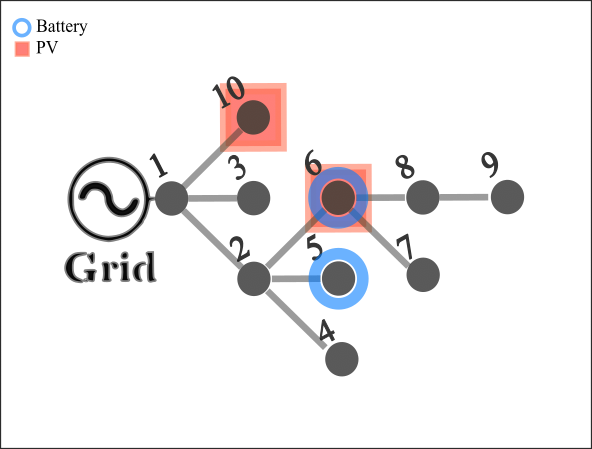
\includegraphics[width=0.6\linewidth]{figures/ads10-pv25-batt25.png}
    \caption{ADS10: 10-bus test system}
    \label{fig:mpopf-tradeoffs-ads10}
\end{figure}

\begin{figure}[h]
    \centering
    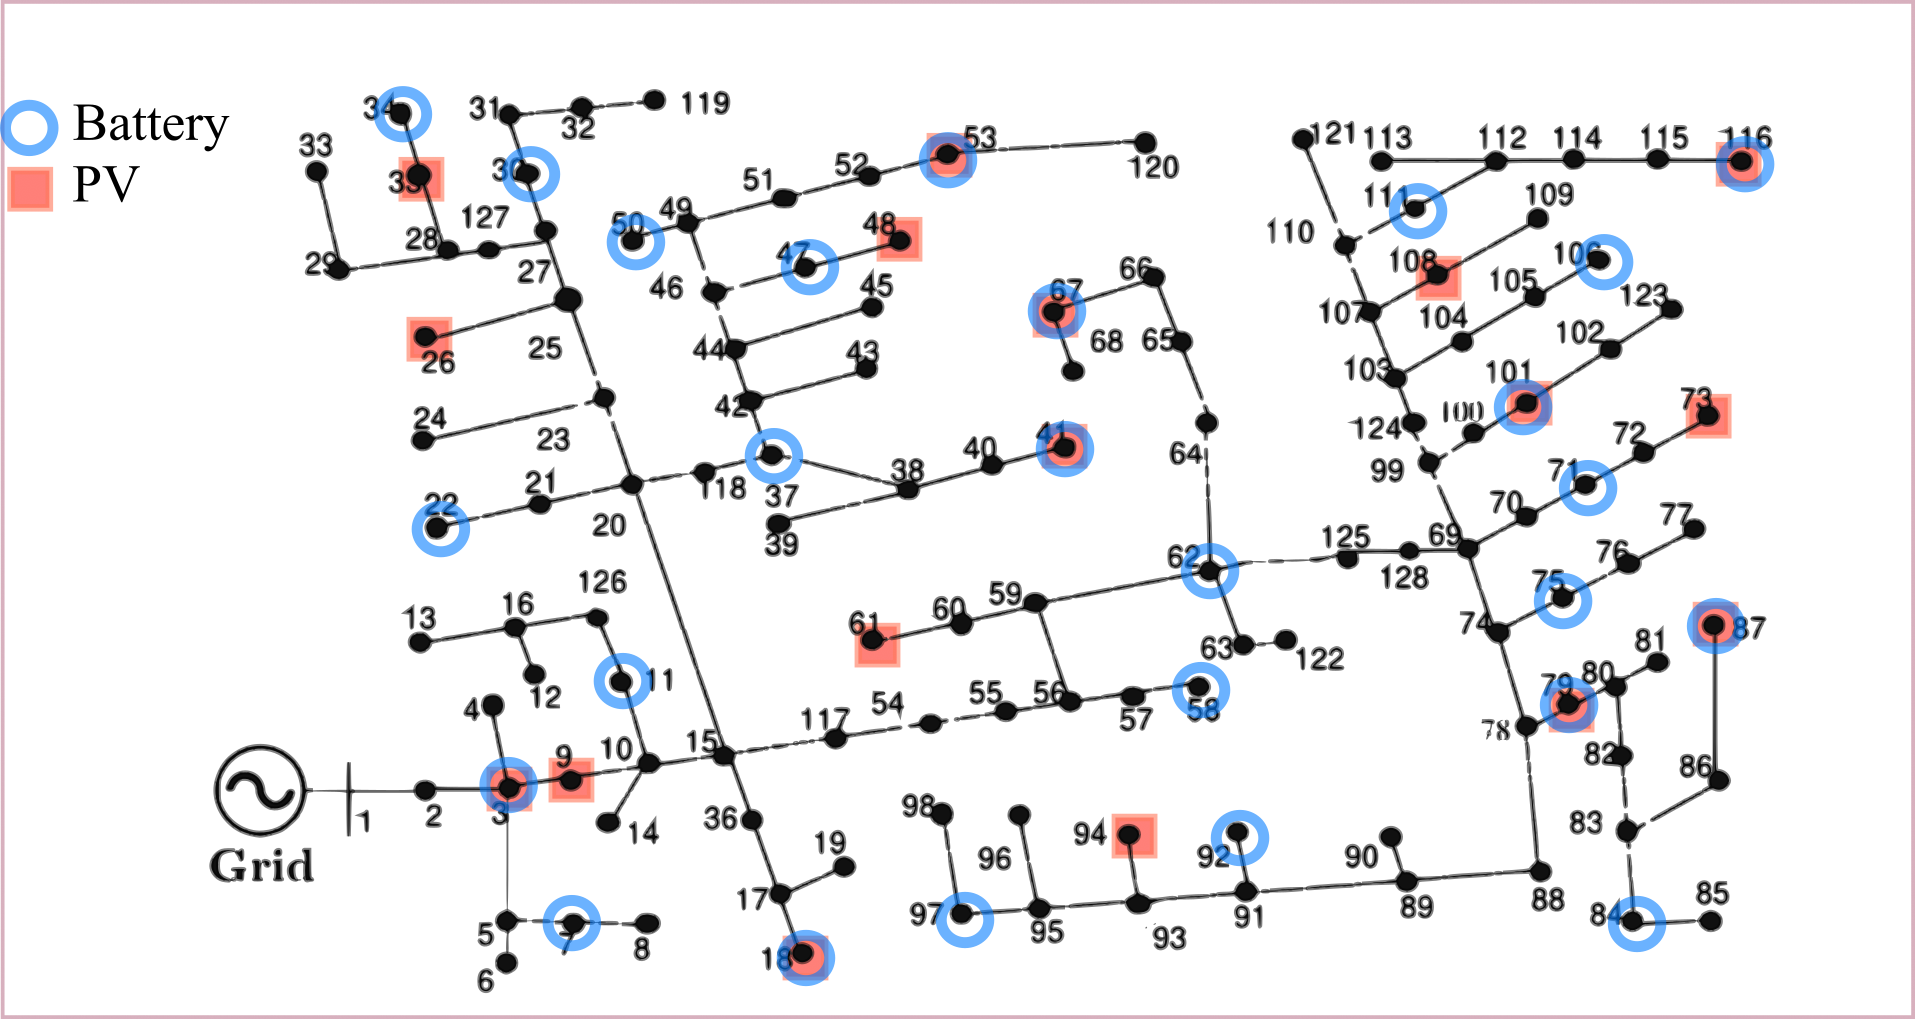
\includegraphics[width=0.85\linewidth]{figures/ieee123-pv20-batt30.png}
    \caption{IEEE-123: 128-bus test system}
    \label{fig:mpopf-tradeoffs-ieee123}
\end{figure}

\Cref{table:mpopf-tradeoffs-system-config} lists configurations. All systems use the 24-hour forecast curves in \Cref{fig:mpopf-tradeoffs-input-curves} with bilevel pricing (peak/off-peak).

\begin{table}[h]
    \centering
    \caption{Test system configurations}
    \label{table:mpopf-tradeoffs-system-config}
    \begin{tabular}{|l|c|c|c|}
    \hline
    \textbf{Parameter} & \textbf{ADS10} & \textbf{IEEE123A} & \textbf{IEEE123B} \\ \hline
    Buses ($n$) & 10 & 128 & 128 \\ \hline
    Load buses ($n_{L}$) & 8 & 85 & 85 \\ \hline
    PV buses ($n_{D}$) & 2 & 17 & 26 \\ \hline
    BESS buses ($n_{B}$) & 2 & 34 & 43 \\ \hline
    GED sizing & 0.33 $p_{L_{R,j}}$ & 0.33 $p_{L_{R,j}}$ & 1.00 $p_{L_{R,j}}$ \\ \hline
    SCD penalty ($\alpha$) & 12.62 & 8.994 & 2.124 \\ \hline
    \end{tabular}
\end{table}

\begin{figure}[h]
    \centering
    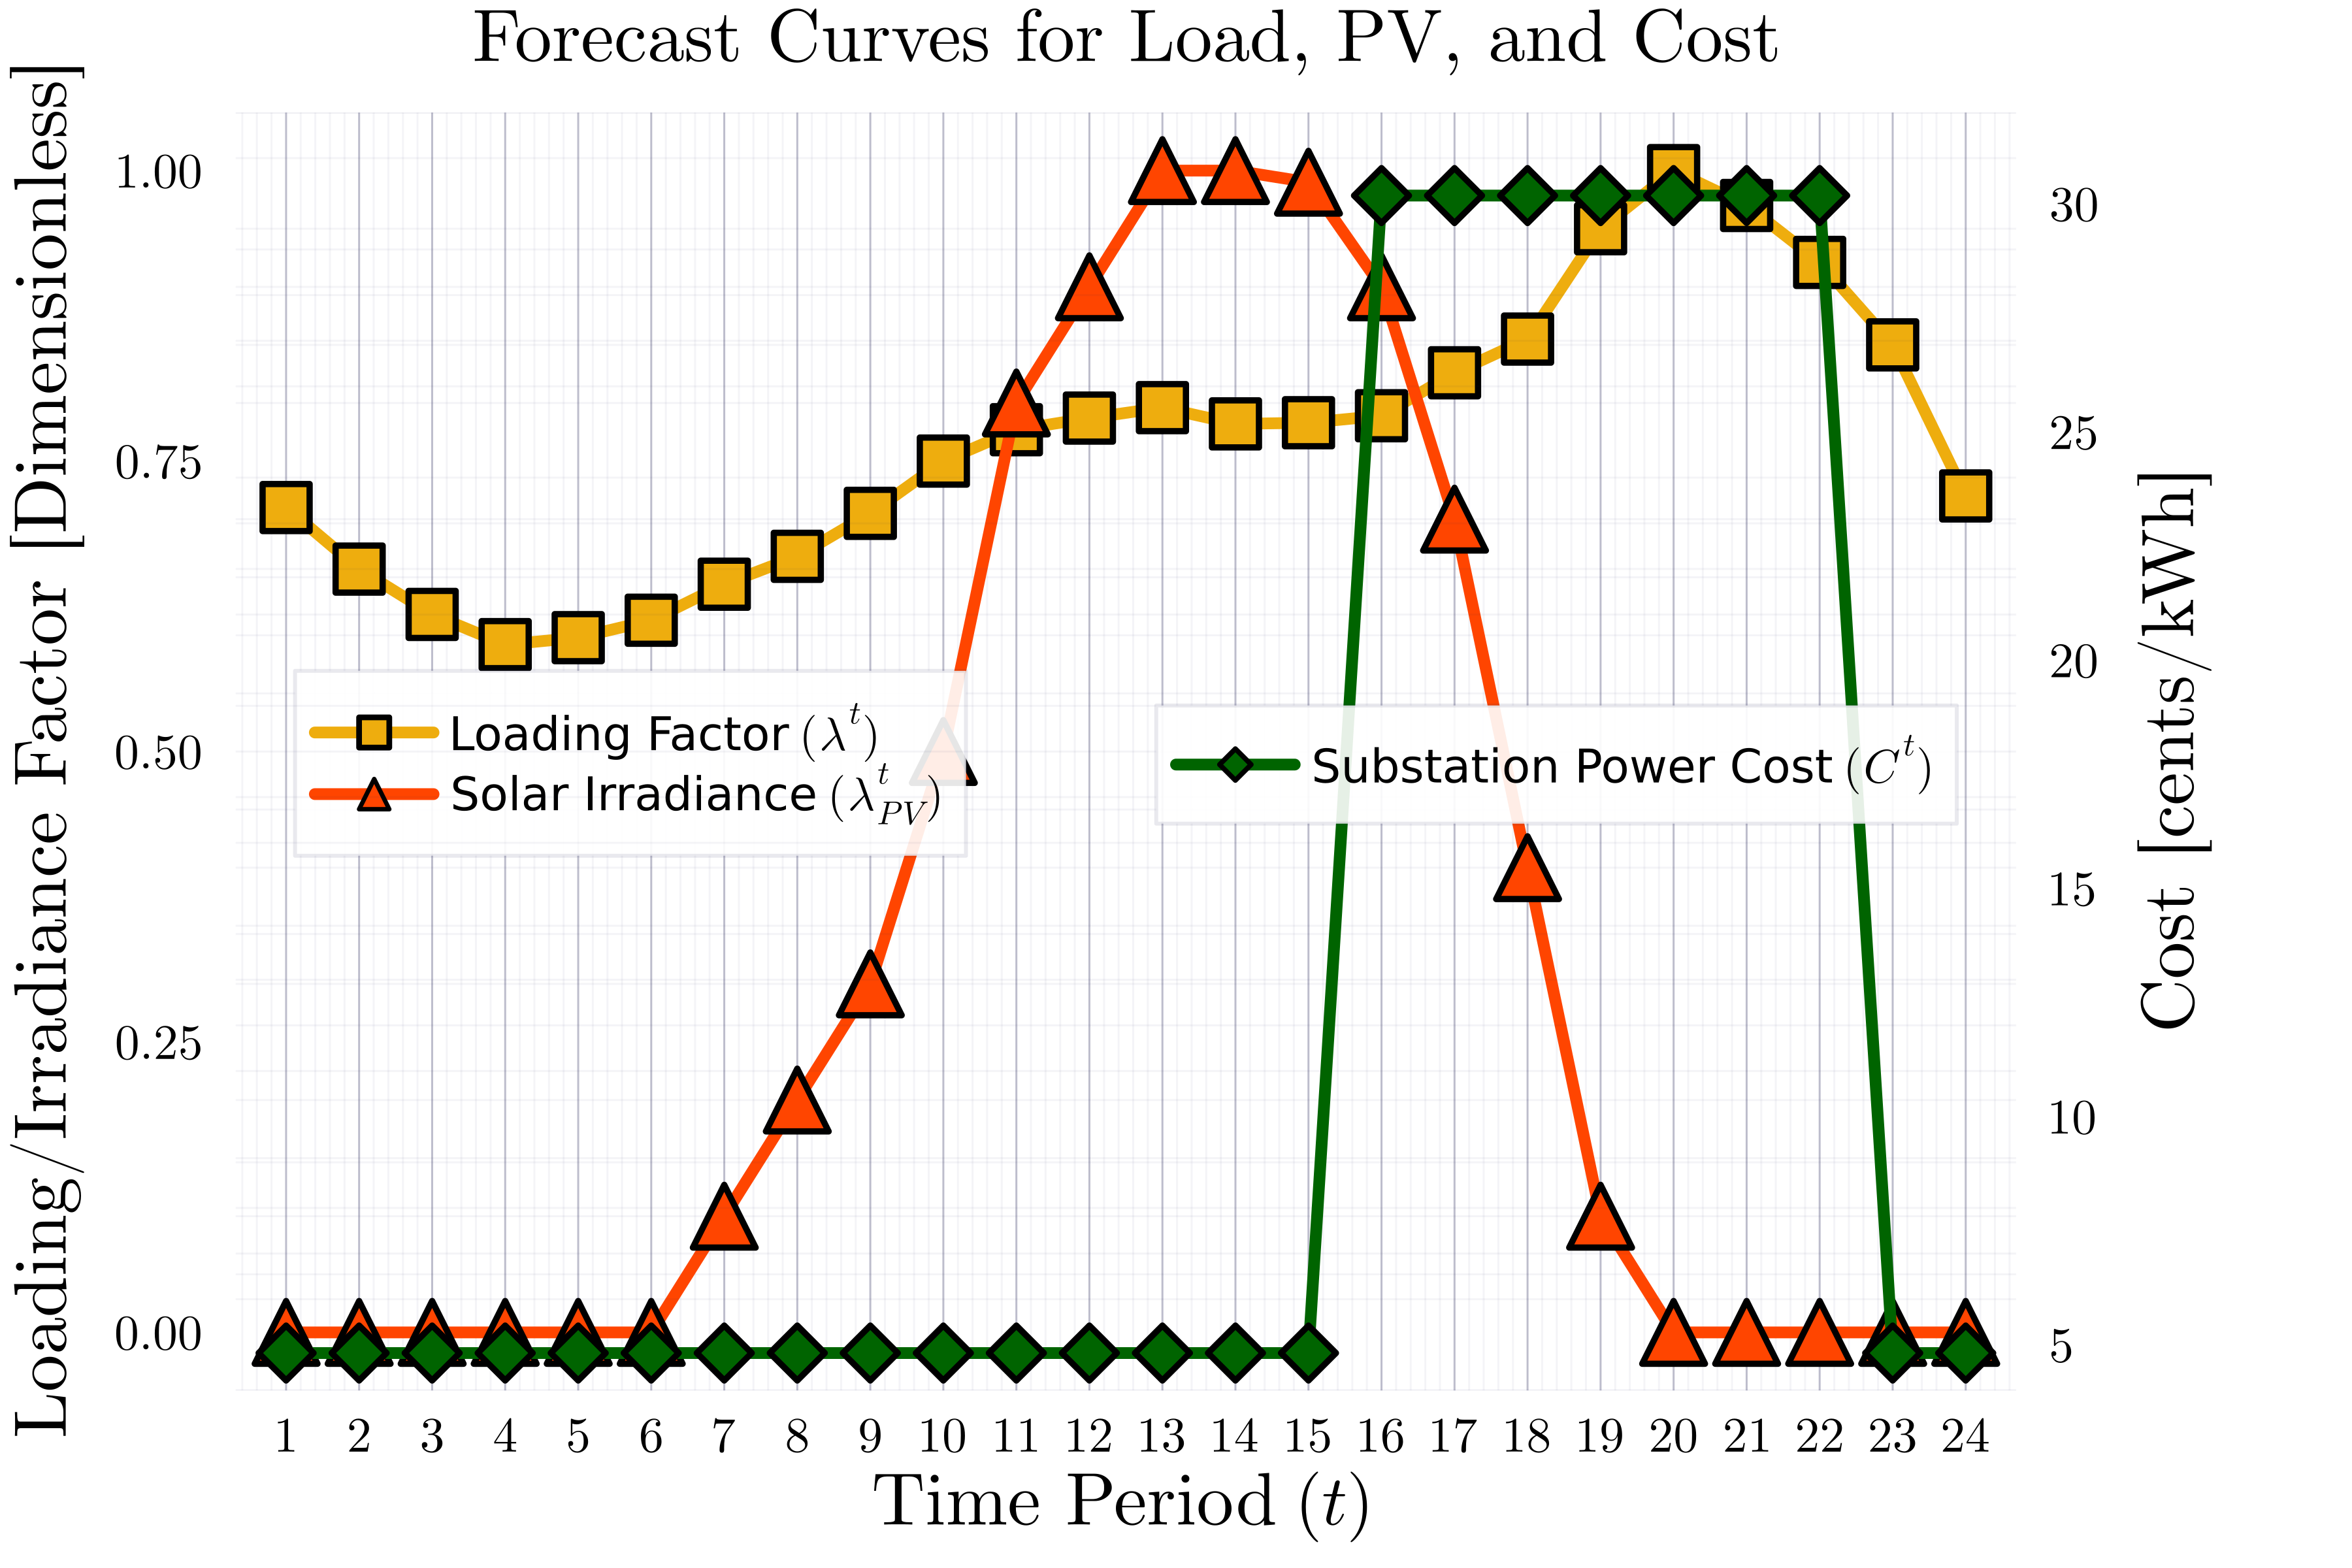
\includegraphics[height=0.22\textheight]{figures/T24-inputCurves/Horizon_24_InputForecastCurves_bilevelCosts.png}
    \caption{24-hour forecasts: load, irradiance, electricity cost}
    \label{fig:mpopf-tradeoffs-input-curves}
\end{figure}

Common parameters: $V_{min}=0.95$ pu, $V_{max}=1.05$ pu, $T=24$ h, $\Delta t=1$ h, $\eta_c=\eta_d=0.95$, $soc_{min}=0.30$, $soc_{max}=0.95$, $B_{R,j} = 4 P_{B_{R,j}}$ (4-hour storage).

\subsubsection{Simulation Workflow}

System data parsed from OpenDSS `.dss' files. Models built in JuMP, solved with Ipopt (cold start for both formulations). Control set-points $(P_{c_j}^t, P_{d_j}^t, q_{B_j}^t, q_{D_j}^t)$ fed back into OpenDSS for AC feasibility validation via OpenDSSDirect.jl \cite{OpenDSSDirect-jl}. Code available at \cite{MPOPFRepo}.

\textbf{Note:} LinDistFlow inherently neglects losses, so reported substation power and losses are from OpenDSS (denoted LinDistFlow$^{\mathbb{O}}$) to ensure fair comparison.

%%%%%%%%%%%%%%%%%%%%%%%%%%%%%%%%%%%%%%%%%%%%%%%%%%%%%%%%%%%%%%%%%%%%%%%%
\subsection{Results}
%%%%%%%%%%%%%%%%%%%%%%%%%%%%%%%%%%%%%%%%%%%%%%%%%%%%%%%%%%%%%%%%%%%%%%%%

%%%%%%%%%%%%%%%%%%%%%%%%%%%%%%%%%%%%%%%%%%%%%%%%%%%%%%%%%%%%%%%%%%%%%%%%
\subsubsection{ADS10 Results}

\begin{table}[H]
    \centering
    \caption{MPOPF performance comparison - ADS10 test system for 24h}
    \label{table:mpopf-tradeoffs-opt-ads10}
    \begin{tabular}{|l|c|c|}
    \hline
    \textbf{Metric} & \textbf{BFM-NL} & \textbf{LinDistFlow\textsuperscript{\(\mathbb{O}\)}} \\ \hline
    \multicolumn{3}{|c|}{\textit{Full horizon}} \\ \hline
    Substation power cost (\$) & 204.27 & 204.28 \\ \hline
    Substation real power (kWh) & 1528.35 & 1528.4 \\ \hline
    Line loss (kWh) & 0.28 & 0.33 \\ \hline
    Substation reactive power (kVARh) & 428.9 & 795.56 \\ \hline
    PV reactive power (kVARh) & 174.41 & -0.69 \\ \hline
    Battery reactive power (kVARh) & 192.8 & -0.37 \\ \hline
    \multicolumn{3}{|c|}{\textit{Computation}} \\ \hline
    Total simulation time (s) & 2.64 & 0.77 \\ \hline
    \end{tabular}
\end{table}

\begin{table}[H]
    \centering
    \caption{MPOPF discrepancy comparison - ADS10 test system for 24h}
    \label{table:mpopf-tradeoffs-feas-ads10}
    \begin{tabular}{|l|c|c|}
    \hline
    \textbf{Metric} & \textbf{BFM-NL} & \textbf{LinDistFlow} \\ \hline
    \multicolumn{3}{|c|}{\textit{Max. all-time discrepancy}} \\ \hline
    Voltage (pu) & 0.00001 & 0.00001 \\ \hline
    Line loss (kW) & 0.000009 & 0.000006 \\ \hline
    Substation power (kW) & 0.000014 & 0.02410 \\ \hline
    Substation reactive power (kVAR) & 0.070706 & 0.05618 \\ \hline
    \end{tabular}
\end{table}

%%%%%%%%%%%%%%%%%%%%%%%%%%%%%%%%%%%%%%%%%%%%%%%%%%%%%%%%%%%%%%%%%%%%%%%%
\subsubsection{IEEE123A Results}

\begin{table}[H]
    \centering
    \caption{MPOPF performance comparison - IEEE123-A test system for 24h}
    \label{table:mpopf-tradeoffs-opt-ieee123a}
    \begin{tabular}{|l|c|c|}
    \hline
    \textbf{Metric} & \textbf{BFM-NL} & \textbf{LinDistFlow\textsuperscript{\(\mathbb{O}\)}} \\ \hline
    \multicolumn{3}{|c|}{\textit{Model dimensions}} \\ \hline
    Decision variables & {15144} & {12096} \\ \hline
    Linear constraints & {18456} & {22200} \\ \hline
    Nonlinear constraints & {3672} & {0} \\ \hline
    \multicolumn{3}{|c|}{\textit{Simulation results}} \\ \hline
    Substation power cost (\$) & 2787.44 & 2798.4 \\ \hline
    Substation real power (kWh) & 20984.89 & 21065.89 \\ \hline
    Line loss (kWh) & 380.09 & 461.38 \\ \hline
    Substation reactive power (kVARh) & 6835.82 & 12259.29 \\ \hline
    PV reactive power (kVARh) & 1972.27 & 195.12 \\ \hline
    Battery reactive power (kVARh) & 3709.71 & 204.63 \\ \hline
    \multicolumn{3}{|c|}{\textit{Computation}} \\ \hline
    Total simulation time (s) & 17.44 & 0.85 \\ \hline
    \end{tabular}
\end{table}

\begin{table}[H]
    \centering
    \caption{MPOPF discrepancy comparison - IEEE123-A test system for 24h}
    \label{table:mpopf-tradeoffs-feas-ieee123a}
    \begin{tabular}{|l|c|c|}
    \hline
    \textbf{Metric} & \textbf{BFM-NL} & \textbf{LinDistFlow} \\ \hline
    \multicolumn{3}{|c|}{\textit{Max. all-time discrepancy}} \\ \hline
    Voltage (pu) & 0.00007 & 0.00206 \\ \hline
    Line loss (kW) & 0.01818 & 1.8074 \\ \hline
    Substation power (kW) & 0.43164 & 32.362 \\ \hline
    Substation reactive power (kVAR) & 1.0102 & 64.403 \\ \hline
    \end{tabular}
\end{table}

%%%%%%%%%%%%%%%%%%%%%%%%%%%%%%%%%%%%%%%%%%%%%%%%%%%%%%%%%%%%%%%%%%%%%%%%
\subsubsection{IEEE123B Results}

\begin{table}[H]
    \centering
    \caption{MPOPF performance comparison - IEEE123-B test system for 24h}
    \label{table:mpopf-tradeoffs-opt-ieee123b}
    \begin{tabular}{|l|c|c|}
    \hline
    \textbf{Metric} & \textbf{BFM-NL} & \textbf{LinDistFlow\textsuperscript{\(\mathbb{O}\)}} \\ \hline
    \multicolumn{3}{|c|}{\textit{Model dimensions}} \\ \hline
    Decision variables & {17184} & {14136} \\ \hline
    Linear constraints & {24168} & {30360} \\ \hline
    Nonlinear constraints & {4080} & {0} \\ \hline
    \multicolumn{3}{|c|}{\textit{Simulation results}} \\ \hline
    Substation power cost (\$) & 1973.83 & 1987.78 \\ \hline
    Substation real power (kWh) & 16594.11 & 16693.01 \\ \hline
    Line loss (kWh) & 234.78 & 333.78 \\ \hline
    Substation reactive power (kVARh) & -404.91 & 11055.41 \\ \hline
    PV reactive power (kVARh) & 7255.22 & 1535.29 \\ \hline
    Battery reactive power (kVARh) & 5371.97 & -190.93 \\ \hline
    \multicolumn{3}{|c|}{\textit{Computation}} \\ \hline
    Total simulation time (s) & 23.75 & 1.66 \\ \hline
    \end{tabular}
\end{table}

\begin{table}[H]
    \centering
    \caption{MPOPF discrepancy comparison - IEEE123-B test system for 24h}
    \label{table:mpopf-tradeoffs-feas-ieee123b}
    \begin{tabular}{|l|c|c|}
    \hline
    \textbf{Metric} & \textbf{BFM-NL} & \textbf{LinDistFlow} \\ \hline
    \multicolumn{3}{|c|}{\textit{Max. all-time discrepancy}} \\ \hline
    Voltage (pu) & 0.000059 & 0.001599 \\ \hline
    Line loss (kW) & 0.00776 & 1.055093 \\ \hline
    Substation power (kW) & 0.217433 & 23.344019 \\ \hline
    Substation reactive power (kVAR) & 1.016894 & 45.925288 \\ \hline
    \end{tabular}
\end{table}

%%%%%%%%%%%%%%%%%%%%%%%%%%%%%%%%%%%%%%%%%%%%%%%%%%%%%%%%%%%%%%%%%%%%%%%%
\subsection{Discussion: Key Insights for Decomposition Algorithms}
%%%%%%%%%%%%%%%%%%%%%%%%%%%%%%%%%%%%%%%%%%%%%%%%%%%%%%%%%%%%%%%%%%%%%%%%

This section synthesizes the simulation results to highlight critical insights that directly inform the choice of formulation for spatial and temporal decomposition algorithms presented in subsequent chapters.

%%%%%%%%%%%%%%%%%%%%%%%%%%%%%%%%%%%%%%%%%%%%%%%%%%%%%%%%%%%%%%%%%%%%%%%%
\subsubsection{Computational Speedup}

As expected, the LinDistFlow model significantly outperforms BFM-NL in computation time, achieving speedups of approximately \textbf{3×, 20×, and 14×} for ADS10, IEEE123A, and IEEE123B systems respectively. This performance gain stems primarily from the elimination of nonlinear constraints (\cref{table:mpopf-tradeoffs-opt-ieee123a,table:mpopf-tradeoffs-opt-ieee123b} show zero nonlinear constraints for LinDistFlow).

Although LinDistFlow may include more total constraints (all linear) than BFM-NL's combination of linear and nonlinear ones, solve times remain dominated by the elimination of nonlinearity. Modern LP solvers handle large numbers of linear constraints efficiently, whereas nonlinear solvers must iteratively navigate non-convex landscapes.

\textbf{Note:} All BFM-NL timings assume a cold start. Warm-starting BFM-NL with LinDistFlow solutions would likely narrow the computational gap further—a strategy worth considering for decomposition algorithms where subproblems are solved repeatedly.

%%%%%%%%%%%%%%%%%%%%%%%%%%%%%%%%%%%%%%%%%%%%%%%%%%%%%%%%%%%%%%%%%%%%%%%%
\subsubsection{Optimality Gap: The Core Tradeoff}

Since the objective function is the cost of total substation power borrowed over the horizon (\(f_0 = \sum_{t=1}^{T} C^t P^t_{Subs} \Delta t\) from \cref{eq:mpopf-tradeoffs-objective}), we quantify the optimality gap as:

\[
\text{Optimality Gap} = \frac{f_{\text{LinDistFlow}} - f_{\text{BFM-NL}}}{f_{\text{BFM-NL}}} \times 100\%
\]

Computing from \cref{table:mpopf-tradeoffs-opt-ads10,table:mpopf-tradeoffs-opt-ieee123a,table:mpopf-tradeoffs-opt-ieee123b}:
\begin{itemize}
    \item \textbf{ADS10}: Gap = 0.005\% (essentially negligible)
    \item \textbf{IEEE123A}: Gap = 0.39\% (acceptable for many applications)
    \item \textbf{IEEE123B}: Gap = 0.71\% (caution required)
\end{itemize}

\textbf{Analysis:} The optimality gap grows with both system size and GED penetration. Two primary factors explain this trend:

\begin{enumerate}
    \item \textbf{Line Loss Approximation}: Larger systems experience greater line losses. LinDistFlow neglects the \((r_{ij}^2 + x_{ij}^2)l_{ij}^t\) term in the KVL equation (\cref{eq:mpopf-tradeoffs-kvl-l} vs \cref{eq:mpopf-tradeoffs-kvl-nl}) and the loss terms in power balance equations (\cref{eq:mpopf-tradeoffs-real-balance-l,eq:mpopf-tradeoffs-reactive-balance-l} vs \cref{eq:mpopf-tradeoffs-real-balance-nl,eq:mpopf-tradeoffs-reactive-balance-nl}). As losses increase, this approximation error compounds.
    
    \item \textbf{Battery Inverter Reactive Power Model}: Higher battery penetration amplifies errors from the hexagonal approximation (\cref{eq:mpopf-tradeoffs-battery-reactive-l}) compared to the true quadratic constraint (\cref{eq:mpopf-tradeoffs-battery-reactive-nl}). This is especially pronounced in IEEE123B where battery ratings equal load ratings (100\% penetration).
\end{enumerate}

\textbf{Implication for Decomposition:} When developing spatial or temporal decomposition algorithms (Chapters~\ref{sec:enapp} and~\ref{sec:tadmm}), using LinDistFlow as the base formulation will propagate this optimality gap. For large-scale systems or high DER penetrations, this gap may be unacceptable. However, for moderate-sized systems with lower penetrations, the computational speedup may justify the small optimality sacrifice.

%%%%%%%%%%%%%%%%%%%%%%%%%%%%%%%%%%%%%%%%%%%%%%%%%%%%%%%%%%%%%%%%%%%%%%%%
\subsubsection{Reactive Power Control: A Critical Discrepancy}

One of the most striking differences between the two formulations is their reactive power management strategy, as seen in the ``PV reactive power'' and ``Battery reactive power'' rows of \cref{table:mpopf-tradeoffs-opt-ads10,table:mpopf-tradeoffs-opt-ieee123a,table:mpopf-tradeoffs-opt-ieee123b}.

\textbf{BFM-NL Behavior:} Deliberately allocates reactive power among PV inverters, batteries, and the substation based on:
\begin{itemize}
    \item Network losses (via the \(l_{ij}^t x_{ij}\) term in \cref{eq:mpopf-tradeoffs-reactive-balance-nl})
    \item Device capabilities and locations
    \item Voltage sensitivity at each bus
\end{itemize}

For example, in IEEE123A (moderate GED penetration), BFM-NL assigns:
\begin{itemize}
    \item 1972 kVARh to PV inverters
    \item 3710 kVARh to battery inverters
    \item 6836 kVARh from substation
\end{itemize}

\textbf{LinDistFlow Behavior:} By dropping the \(l_{ij}^t x_{ij}\) term (\cref{eq:mpopf-tradeoffs-reactive-balance-l}), LinDistFlow loses sensitivity to how reactive power dispatch affects line losses. Consequently, it assigns reactive power in an almost arbitrary manner—often defaulting most reactive support to the substation:
\begin{itemize}
    \item 195 kVARh to PV inverters (10× less than BFM-NL)
    \item 205 kVARh to battery inverters (18× less than BFM-NL)
    \item 12259 kVARh from substation (1.8× more than BFM-NL)
\end{itemize}

\textbf{Practical Consequences:}
\begin{enumerate}
    \item \textbf{Under-utilization of Distributed Assets}: LinDistFlow fails to leverage the reactive power capability of distributed inverters, missing opportunities for localized voltage support and loss reduction.
    
    \item \textbf{Substation Overload Risk}: Concentrating reactive power at the substation may violate transformer ratings or lead to inefficient operation.
    
    \item \textbf{Voltage Profile Degradation}: While both models achieve similar substation costs, LinDistFlow's coarse reactive dispatch risks larger voltage deviations throughout the network, especially during contingencies.
    
    \item \textbf{Missed Grid Support Opportunities}: Modern grid codes increasingly require DERs to provide reactive support. LinDistFlow-based control strategies would systematically under-utilize this capability.
\end{enumerate}

\textbf{Implication for Decomposition:} If the objective function includes voltage regulation, reactive power costs, or inverter utilization penalties (beyond simple substation cost minimization), LinDistFlow-based decomposition algorithms will produce fundamentally flawed solutions. Even for cost-minimization objectives, the reactive power mismatch creates operational risks that may be unacceptable in practice.

%%%%%%%%%%%%%%%%%%%%%%%%%%%%%%%%%%%%%%%%%%%%%%%%%%%%%%%%%%%%%%%%%%%%%%%%
\subsubsection{Voltage and Power Feasibility}

\Cref{table:mpopf-tradeoffs-feas-ads10,table:mpopf-tradeoffs-feas-ieee123a,table:mpopf-tradeoffs-feas-ieee123b} quantify discrepancies when control set-points from each model are applied in OpenDSS. These are computed as:

\[
\text{Disc}_v = \max_{j \in \mathcal{N}, t \in \tau} |V^t_{j,\text{OpenDSS}} - V^t_{j,\text{model}}|
\]
\[
\text{Disc}_{P_{Subs}} = \max_{t \in \tau} |P^t_{Subs,\text{OpenDSS}} - P^t_{Subs,\text{model}}|
\]

\textbf{Voltage Deviation:} LinDistFlow maintains voltage errors under \textbf{0.2\%} compared to BFM-NL (which itself has negligible errors). For most distribution operations, this is acceptable and unlikely to cause voltage limit violations.

\textbf{Substation Power Underprediction:} This is the critical concern. LinDistFlow can under-predict hourly substation power by up to \textbf{2--5\%} (24--32 kW for IEEE123A, which represents hundreds of kWh over the horizon). This creates three operational risks:

\begin{enumerate}
    \item \textbf{Equipment Limit Violations}: If the actual substation draw approaches transformer ratings, LinDistFlow's underestimation may lead to overloads.
    
    \item \textbf{Reserve Margin Errors}: System operators rely on accurate power predictions to maintain adequate reserves. A 5\% error can compromise reliability during contingencies.
    
    \item \textbf{Economic Inaccuracies}: In real-time markets, substation power ties directly to settlement costs. Systematic underprediction leads to unexpected charges and missed arbitrage opportunities.
\end{enumerate}

\textbf{Implication for Decomposition:} When using LinDistFlow-based decomposition, the subproblem solutions will consistently underestimate substation power and line losses. Aggregating these errors across spatial regions or temporal windows can produce dangerously optimistic predictions. Post-processing corrections or warm-starting with LinDistFlow followed by BFM-NL refinement becomes essential.

%%%%%%%%%%%%%%%%%%%%%%%%%%%%%%%%%%%%%%%%%%%%%%%%%%%%%%%%%%%%%%%%%%%%%%%%
\subsubsection{Complementary Modeling Strategy: A Hybrid Approach}

Based on the above analysis, a purely LinDistFlow-based or purely BFM-NL-based approach each has critical limitations:

\textbf{LinDistFlow Strengths:}
\begin{itemize}
    \item Fast convergence (10--20× speedup)
    \item Near-optimal cost objective (within 0.4--0.7\% for moderate systems)
    \item Suitable for rapid scenario screening or initialization
\end{itemize}

\textbf{LinDistFlow Weaknesses:}
\begin{itemize}
    \item Under-reports substation power and line losses
    \item Arbitrary reactive power allocation
    \item Optimality gap grows with system size and GED penetration
\end{itemize}

\textbf{BFM-NL Strengths:}
\begin{itemize}
    \item Accurate physics representation
    \item Physically consistent control and state variables
    \item Intelligent reactive power dispatch
\end{itemize}

\textbf{BFM-NL Weaknesses:}
\begin{itemize}
    \item Slow convergence (especially for cold starts)
    \item May struggle with large-scale systems without decomposition
\end{itemize}

\paragraph{Recommended Hybrid Strategy:}

For the spatial and temporal decomposition algorithms developed in subsequent chapters, we recommend:

\begin{enumerate}
    \item \textbf{Phase 1 (Initialization)}: Solve the MPOPF problem using LinDistFlow to quickly obtain near-optimal control set-points. Use these to warm-start the subsequent phase.
    
    \item \textbf{Phase 2 (Refinement)}: Solve the MPOPF problem using BFM-NL, initialized with Phase 1 results. This captures accurate physics while benefiting from the warm start to reduce computation time.
    
    \item \textbf{Phase 3 (Validation)}: Always validate final control set-points through OpenDSS or another AC power flow solver before deployment.
\end{enumerate}

This hybrid approach provides a \textbf{feasible and optimal solution suitable for real-time operations} while maintaining computational tractability. The spatial decomposition (ENApp) and temporal decomposition (ADMM) algorithms presented in the following chapters can incorporate either formulation or this hybrid strategy depending on the application requirements.

%%%%%%%%%%%%%%%%%%%%%%%%%%%%%%%%%%%%%%%%%%%%%%%%%%%%%%%%%%%%%%%%%%%%%%%%
\subsection{Conclusions and Implications}

This chapter has demonstrated that the choice of power flow formulation—before any decomposition is attempted—has profound implications for solution quality, computational efficiency, and operational feasibility. The key findings are:

\begin{enumerate}
    \item \textbf{Optimality Gap}: LinDistFlow introduces a gap that grows from 0.005\% (small systems) to 0.7\% (large systems with high GED penetration). While acceptable for cost minimization in moderate-sized systems, this gap may be unacceptable for large-scale deployments.
    
    \item \textbf{Reactive Power Mismanagement}: LinDistFlow systematically under-utilizes distributed inverter assets, concentrating reactive power at the substation. This creates operational risks and misses grid support opportunities.
    
    \item \textbf{Substation Power Underprediction}: LinDistFlow can underestimate hourly substation power by up to 5\%, risking equipment overloads, reserve margin violations, and economic inaccuracies.
    
    \item \textbf{Computational Speedup}: LinDistFlow achieves 10--20× faster solve times by eliminating nonlinear constraints, making it attractive for rapid scenario analysis or warm-start initialization.
\end{enumerate}

\textbf{Central Insight:} \textit{The formulation you choose fundamentally shapes the behavior of any decomposition algorithm built on top of it.} A spatially or temporally decomposed MPOPF using LinDistFlow will inherit its reactive power mismanagement and substation power errors, even if the decomposition itself converges correctly. Conversely, a decomposed BFM-NL approach will be more computationally expensive but will produce physically consistent and operationally sound solutions.

\textbf{Forward Connection:} The subsequent chapters develop:
\begin{itemize}
    \item \textbf{Chapter on Spatial Decomposition (ENApp)}: A spatially distributed MPOPF algorithm that partitions the network into areas. The insights from this chapter inform whether to use BFM-NL, LinDistFlow, or a hybrid approach for the area subproblems.
    
    \item \textbf{Chapter on Temporal Decomposition (tADMM)}: An ADMM-based temporal decomposition that breaks the multi-period problem into single-period subproblems. The formulation choice (BFM-NL vs LinDistFlow) directly affects convergence behavior and solution quality.
\end{itemize}

By carefully considering the tradeoffs analyzed in this chapter, the decomposition algorithms can be designed to balance computational efficiency with solution accuracy, ultimately enabling scalable and reliable MPOPF for modern distribution networks with high penetrations of grid edge devices.
